\chapter{疾病标记物的自动定位方法}\label{sec:method}
有鉴目前已有的相关工作无法实现疾病标记物的精确定位(相关内容参见\ref{sec:related_work}小节),本文将提出一种新颖的网络模型和训练方法,以期达到精确定位疾病标记物的目的。具体而言,在\ref{sec:idea_thinking}小节,本文将叙述本文的研究问题和我们的解决思路。接着,在\ref{sec:model_architecture_intro}小节中,本文将介绍模型结构,包括各个子模块和各自充当的角色。最后,我们将在\ref{sec:loss_func_training_stragies}小节中定义损失函数、训练步骤以及网络更新策略。

\section{研究问题与解决思路}\label{sec:idea_thinking}
\subsection{研究问题}
在医学图像中,疾病标记物具有极强的临床应用价值,可用于处理疾病诊断、疾病风险预测、疾病类型区分等问题,精确定位疾病标记物是其关键一步。在医学图像中,如果疾病标记物分布广泛,边界模糊,尺寸大小与数量不一,医生很难甚至不可能精确标出疾病标记物的位置。仅仅依靠图像级标注来定位疾病标记物更具可行性。鉴于以上情况,本文旨在在弱监督条件下精确定位医学图像中分布广泛、边界模糊、尺寸大小与数量不一的疾病标记物。
\subsection{解决思路}
面对弱监督条件下,疾病标记物的精确定位这一问题,鉴于已有方法只能粗略定位到疾病标记物,我们可用生成对抗网络思路去做,保证输入输出图像尺寸相等,以避免上采样所带来的定位不够精确的问题。我们期望本文设计的GAN具有以下能力:

1)如果输入图像是正常图像,那么GAN中的生成器输出图像与输入图像保持一致,即此时输入图像中并没有像素强度发生改变。
	
2)如果输入图像是异常图像,可以想象,如果GAN中的生成器输出图像与输入图像相比,只有极少数像素强度发生改变,而绝大部分像素强度没有发生改变,那么我们完全有理由认为这些发生改变了的像素便是疾病标记物,此时我们可以认为GAN中的生成器的输出图像是异常输入图像去除疾病标记物之后的“正常”版本,则疾病标记物的准确位置可由GAN中的生成器的输出图像减去输入图像给出。

\noindent 一旦GAN具有以上功能,我们就可以很好地定位图像中的疾病标记物。考虑到GAN能较好地去除图像中的遮挡物,比如,GAN去除图像中的雨滴~\cite{qian2018attentive}(见图\ref{subfig:attention_gan}),GAN去除人脸中的遮挡物~\cite{yuan2019face}(见图\ref{subfig:face_de_occulusion})。特别地,对于雨滴这种相对较小、分布较为广泛的物体,GAN仍能处理得相当好,这足以证明GAN强大的图像生成能力,我们完全可借助GAN的出色图像生成能力来去除医学图像中相对较小、广泛分布的疾病标记物。
\begin{figure}[h!]
	\begin{subfigure}{0.45\textwidth}
		\centering
		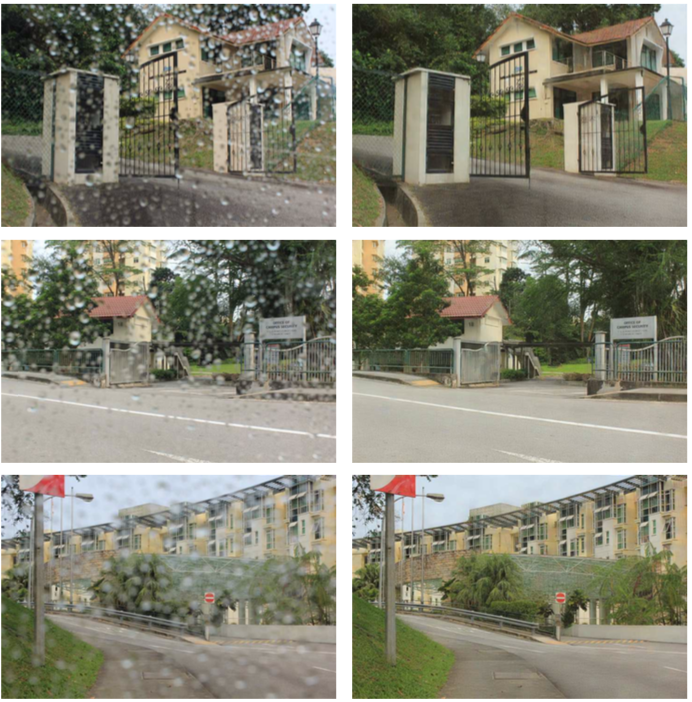
\includegraphics[width=0.75\textwidth]{figure/attention_gan_example.png}
		\caption{GAN去除图像中的雨滴~\cite{qian2018attentive}。}
		\label{subfig:attention_gan}
	\end{subfigure}
	\begin{subfigure}{0.45\textwidth}
		\centering
		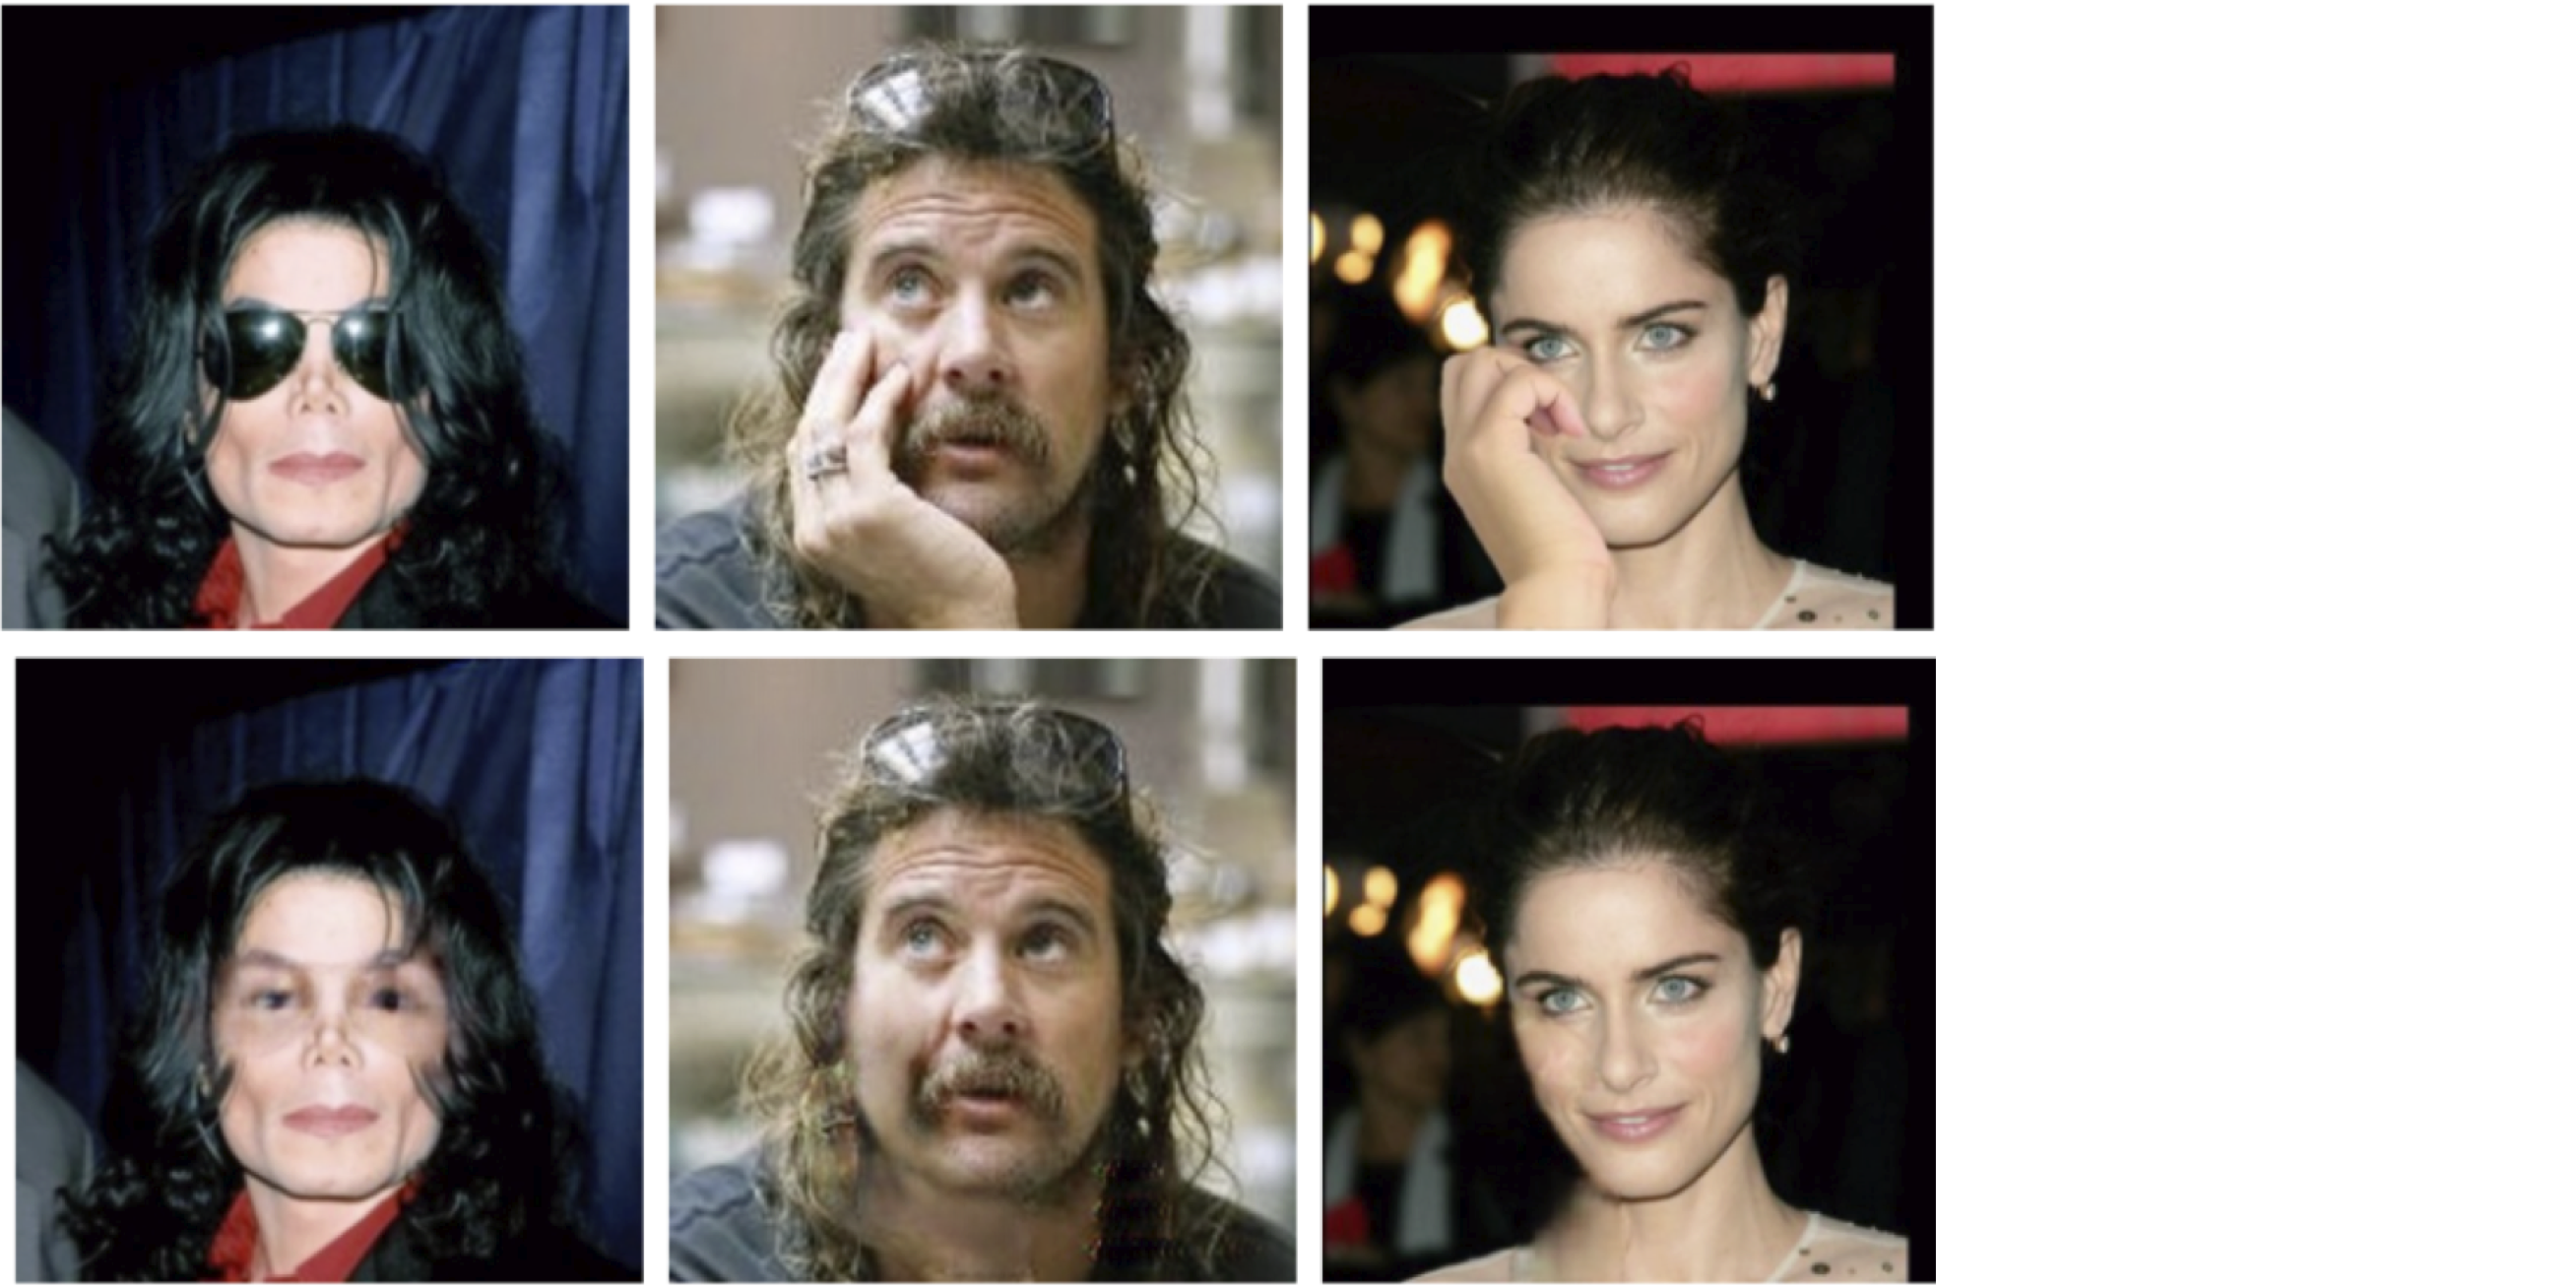
\includegraphics[width=1.5\textwidth]{figure/face_de_occulusion.png}
		\caption{GAN去除人脸图像中的遮挡物~\cite{yuan2019face}。}
		\label{subfig:face_de_occulusion}
	\end{subfigure}
	\caption[GAN去除图像中的遮挡物示例]{GAN去除图像中的遮挡物示例(图片均来自于对应原文~\cite{qian2018attentive,yuan2019face})。}
	\label{mul_fig:gan_auto_encoder_example}
\end{figure}
\section{模型结构介绍}\label{sec:model_architecture_intro}
在\ref{sec:idea_thinking}小节中,本文已经介绍了定位疾病标记物的解决思路和理论建模。本小节内容将详细介绍本文提出的疾病标记物定位模型及其各个子模块的模型结构,力求读者能清晰明了地理解本文提出的方法。
\subsection{疾病标记物自动定位模型}\label{subsec:model_architecture}
本文提出的模型的目的是仅仅使用图像级别的标签,精确定位异常图像中的疾病标记物。我们的想法是设计一种自动学习识别并定位疾病标记物的新模型。出于这种目的,我们提出了一种新颖的深度神经网络。这种网络极具创造性地结合了两种不同的深度学习模型(见图\ref{fig:our_model_architecture}):发挥监督作用的CNN分类器和负责图像生成的GAN(由编码器-解码器和判别器组成)。CNN分类器和判别器可以共同帮助编码器-解码器更有效地去除输入图像中的疾病标记物。训练完成后,可以通过编码器-解码器的输入减去其输出来定位疾病标记物。
\begin{figure}[h]
	\centering
	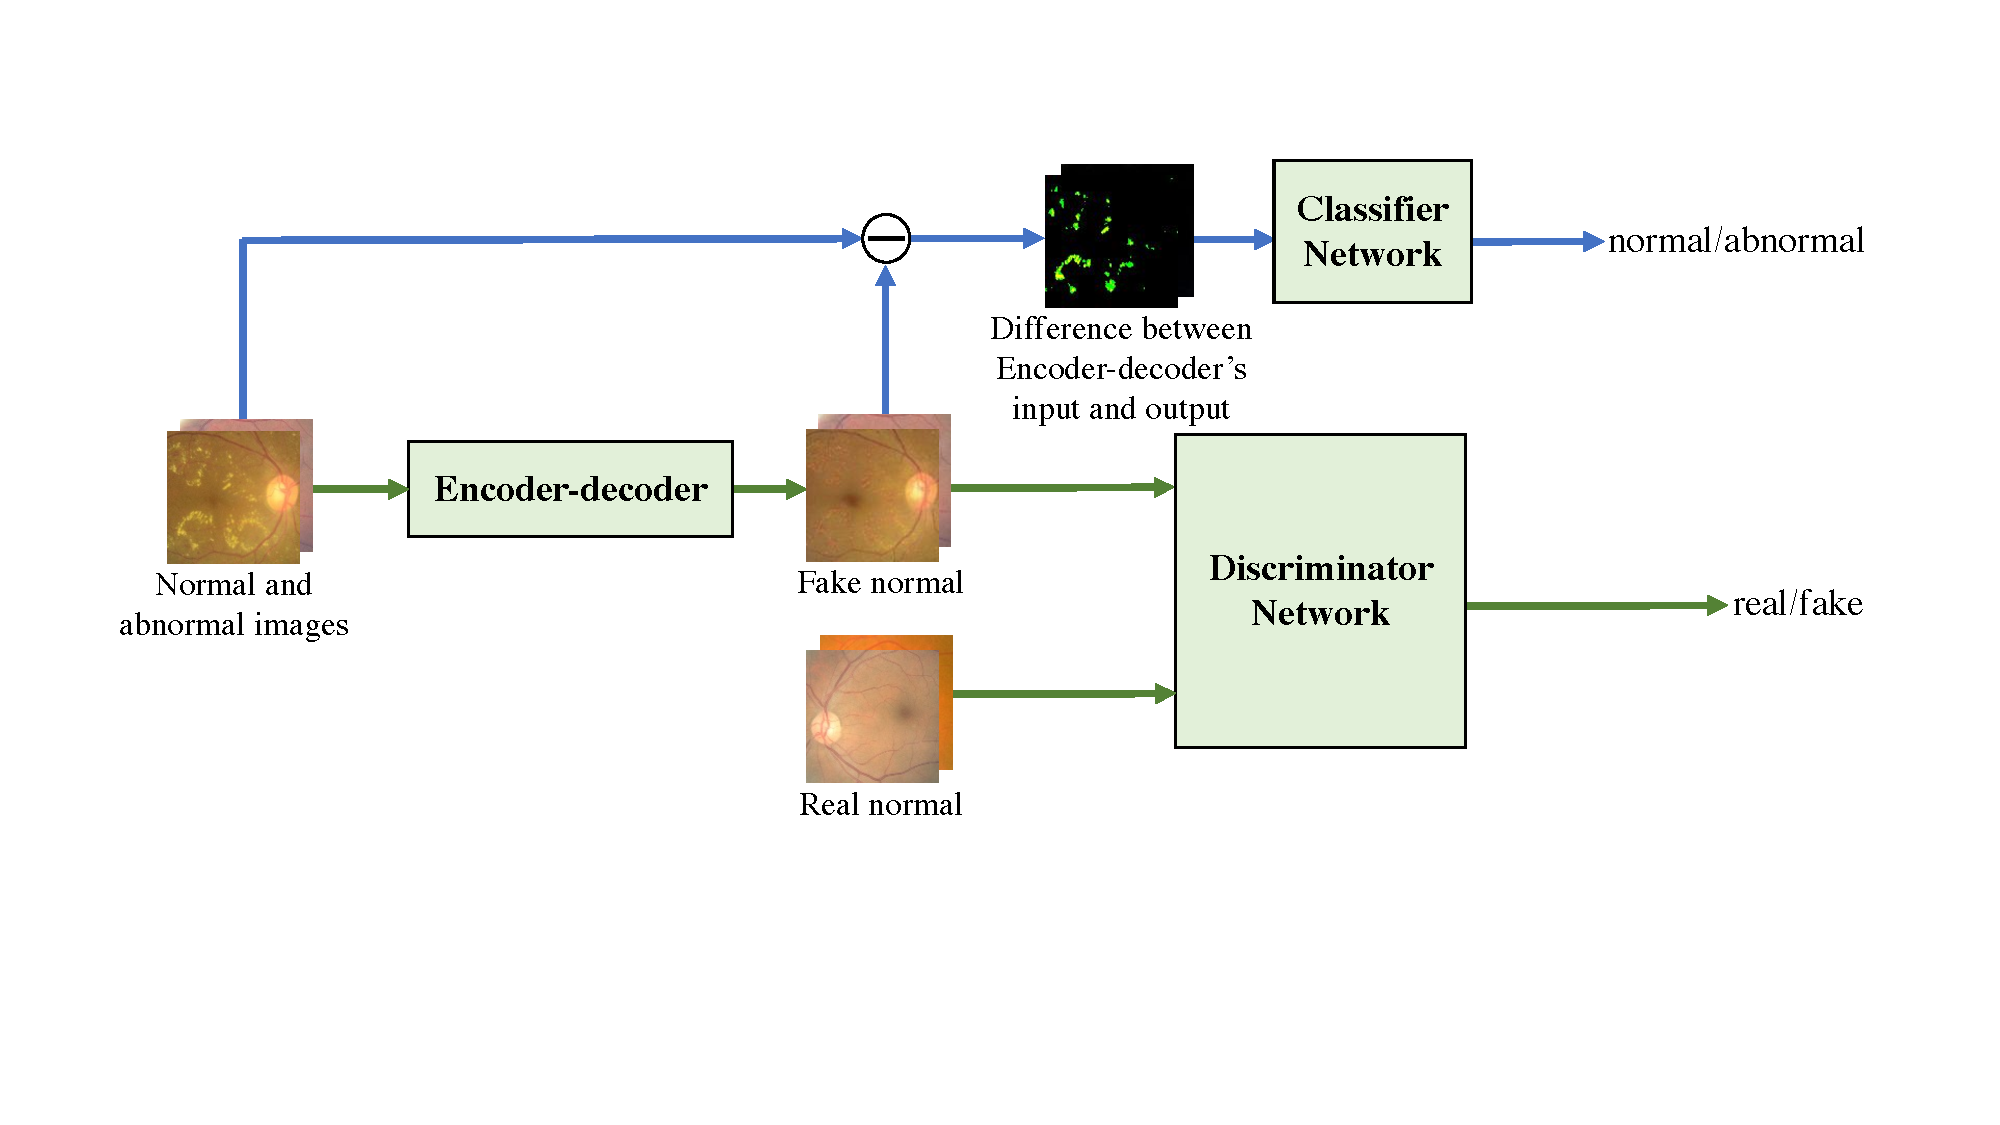
\includegraphics[width=1.0\textwidth]{figure/method.pdf}
	\caption[本文提出的疾病标记物自动定位网络]{本文提出的疾病标记物自动定位网络。} 
	\label{fig:our_model_architecture}
\end{figure}
在提出的模型中,编码器-解码器尝试从输入图像中去除任何疾病标记物,为异常的输入图像生成伪造的正常图像,或者在输入正常图像的情况下保持输出图像与输入相同。通过输入图像减去对应的编码器-解码器输出,就可以轻松地对任何疾病标记物进行定位和分割。尽管可以仅使用正常图像来训练这种编码器-解码器,但这并没有利用现有的异常图像,因此不能直接学习到疾病标记物的特征以进行定位。取而代之的是,为了更有效地实现编码器-解码器的目标,我们在编码器-解码器的顶部添加了CNN分类器,其中CNN分类器的输入是GAN中的编码器-解码器的输入减去对应输出,而CNN分类器的监督信号仍是是原始输入图像的类别标签。为了准确地对图像进行分类,CNN分类器与编码器-解码器必须将异常图像与正常图像区分开。理想情况下,如果CNN分类器的输入仅包含异常原始图像的疾病标记物,而对于正常图像则不包含任何疾病标记物(各处均为零),则CNN分类器将能更准确地、更完美地预测CNN输入的类别标签。换句话说,训练更准确的CNN分类器可以帮助编码器-解码器保持正常区域,从而使CNN分类器的输入仅包含疾病标记物的信号。

但是,CNN分类器可能会帮助编码器-解码器仅从原始输入图像中定位部分疾病标记物。这是因为定位来自原始异常图像的部分疾病标记物信号足以使CNN分类器轻松区分正常图像和异常图像。在这种情况下,编码器-解码器的输出中仍将包含一些疾病标记物。为了进一步帮助编码器-解码器从原始异常图像中删除潜在的疾病标记物,我们添加了一个判别器来判断编码器-解码器的输出是否看起来像真实的正常图像。通过强制编码器-解码器的输出看起来更像正常图像,判别器可帮助编码器-解码器从原始图像中去除尽可能多的疾病标记物信号。

显然,编码器-解码器和判别器一起形成了生成对抗网络。读者可能会认为,在架构中没有CNN分类器的生成对抗网络本身足以帮助编码器-解码器从图像中去除潜在的疾病标记物。但是,生成对抗网络本身可能会提供过多帮助,以至于编码器-解码器生成的图像过于正常,但与输入相比,编码器-解码器输出的正常区域也会不可避免地发生改变。在这种情况下,编码器-解码器的输出与其输入相减(即CNN分类器的输入)会同时包含正常信号和疾病标记物信号,这又使CNN分类器将异常图像与正常图像区分开来相对较困难。这意味着CNN分类器和判别器应该一起工作以帮助编码器-解码器去除潜在的疾病标记物,即判别器帮助编码器-解码器输出正常图像,而CNN分类器帮助编码器-解码器仅改变疾病标记物区域以生成正常输出。我们在后文实验中也证实了这一点(参见第\ref{sec:experiments}章相关内容)。

到此,我们阐述了整体模型及其子模块(编码器-解码器、CNN分类器和判别器)所起的作用,接下来本文将介绍以上三个子模块的模型结构。

\subsection{编码器-解码器}\label{subsec:encoder_decoder_model}
编码器-解码器在GAN中充当生成器的角色,编码器-解码器的训练结果决定了本文提出的方法的疾病标记物定位性能。本文决定在U-Net的基础上进行微调得到本文使用的编码器-解码器,将U-Net迁移到本任务上来。原因主要有以下三点:

1)近些年来,U-Net在医学影像分析领域的应用越来越广泛,无论是在处理图像分割任务上~\cite{oktay2018attention, dong2017automatic},还是在把U-Net当做生成器与其他判别器来组成生成对抗网络~\cite{Han2018SpineGANSS}上,U-Net都表现不俗、性能出色。

2)在疾病标记物的精确定位任务中,只需要极少像素强度发生改变,而其他绝大部分像素都需要较好地重建出来,而U-Net的跨层结构能够很好地将编码阶段的特征融合到解码阶段,有利于图像尤其是具有丰富细节纹理的图像的重建。

3)U-Net是全卷积网络的一种,可允许任意尺寸大小的图像输入,这增加了输入图像输入尺寸的灵活性,上/下采样的次数也可由U-Net的深度灵活控制。另外,由于跨层的存在,梯度回传也比较容易,训练过程中不容易出现梯度消失情况。

因此,本文选用U-Net为基本骨架,将U-Net迁移到本文任务上来。与原始U-Net相比,本文编码器-解码器在模型结构方面作出了两点调整:

1)在编码阶段,为了尽可能减少下采样过程中造成的信息丢失,本文编码器-解码器中使用卷积(卷积核大小为3$\times$3,步长为2)代替最大池化层。相应的,在解码阶段,本文编码器-解码器中使用反卷积(卷积核大小为2$\times$2,步长为2)实现上采样。

2)由于本文编码器-解码器的输入图像经过预处理之后的范围为[-1,1],在最后一个1$\times$1卷积之后,本文编码器-解码器使用Tanh激活函数替代Sigmod激活函数。

经过以上微调后,图\ref{fig:auto_encoder_architecture}展示了本文编码器-解码器的最终网络结构。输入图像尺寸为128$\times$128,网络下采样次数为4。可以看出,编码器-解码器是以U-Net为骨架,编码阶段和解码阶段在网络结构上仍呈现“U”形。在编码阶段,随着深度的增加,特征图尺寸逐步减小,通道数或者说卷积核数量逐渐增加,直到到达最底层。与编码阶段相反,解码阶段随着深度减少,特征图尺寸逐步增大,通道数或者卷积核数量逐渐减小,同时来自编码阶段的特征不断通过跨层结构被融合到解码阶段的特征中,直到到达最顶层,随后经过一个卷积核大小为1$\times$1、步长为1的卷积层,将通道数降低至和输入图像一致,最后特征图经过Tanh激活函数后作为网络输出。编码器-解码器实际上通过编码阶段和解码阶段完成了对输入图像的重建过程,并保证了输入维度和输出维度相同。CNN分类器和判别器一起帮助编码器-解码器通过编码过程和解码过程去除疾病标记物。
\begin{figure}[h]
	\centering
	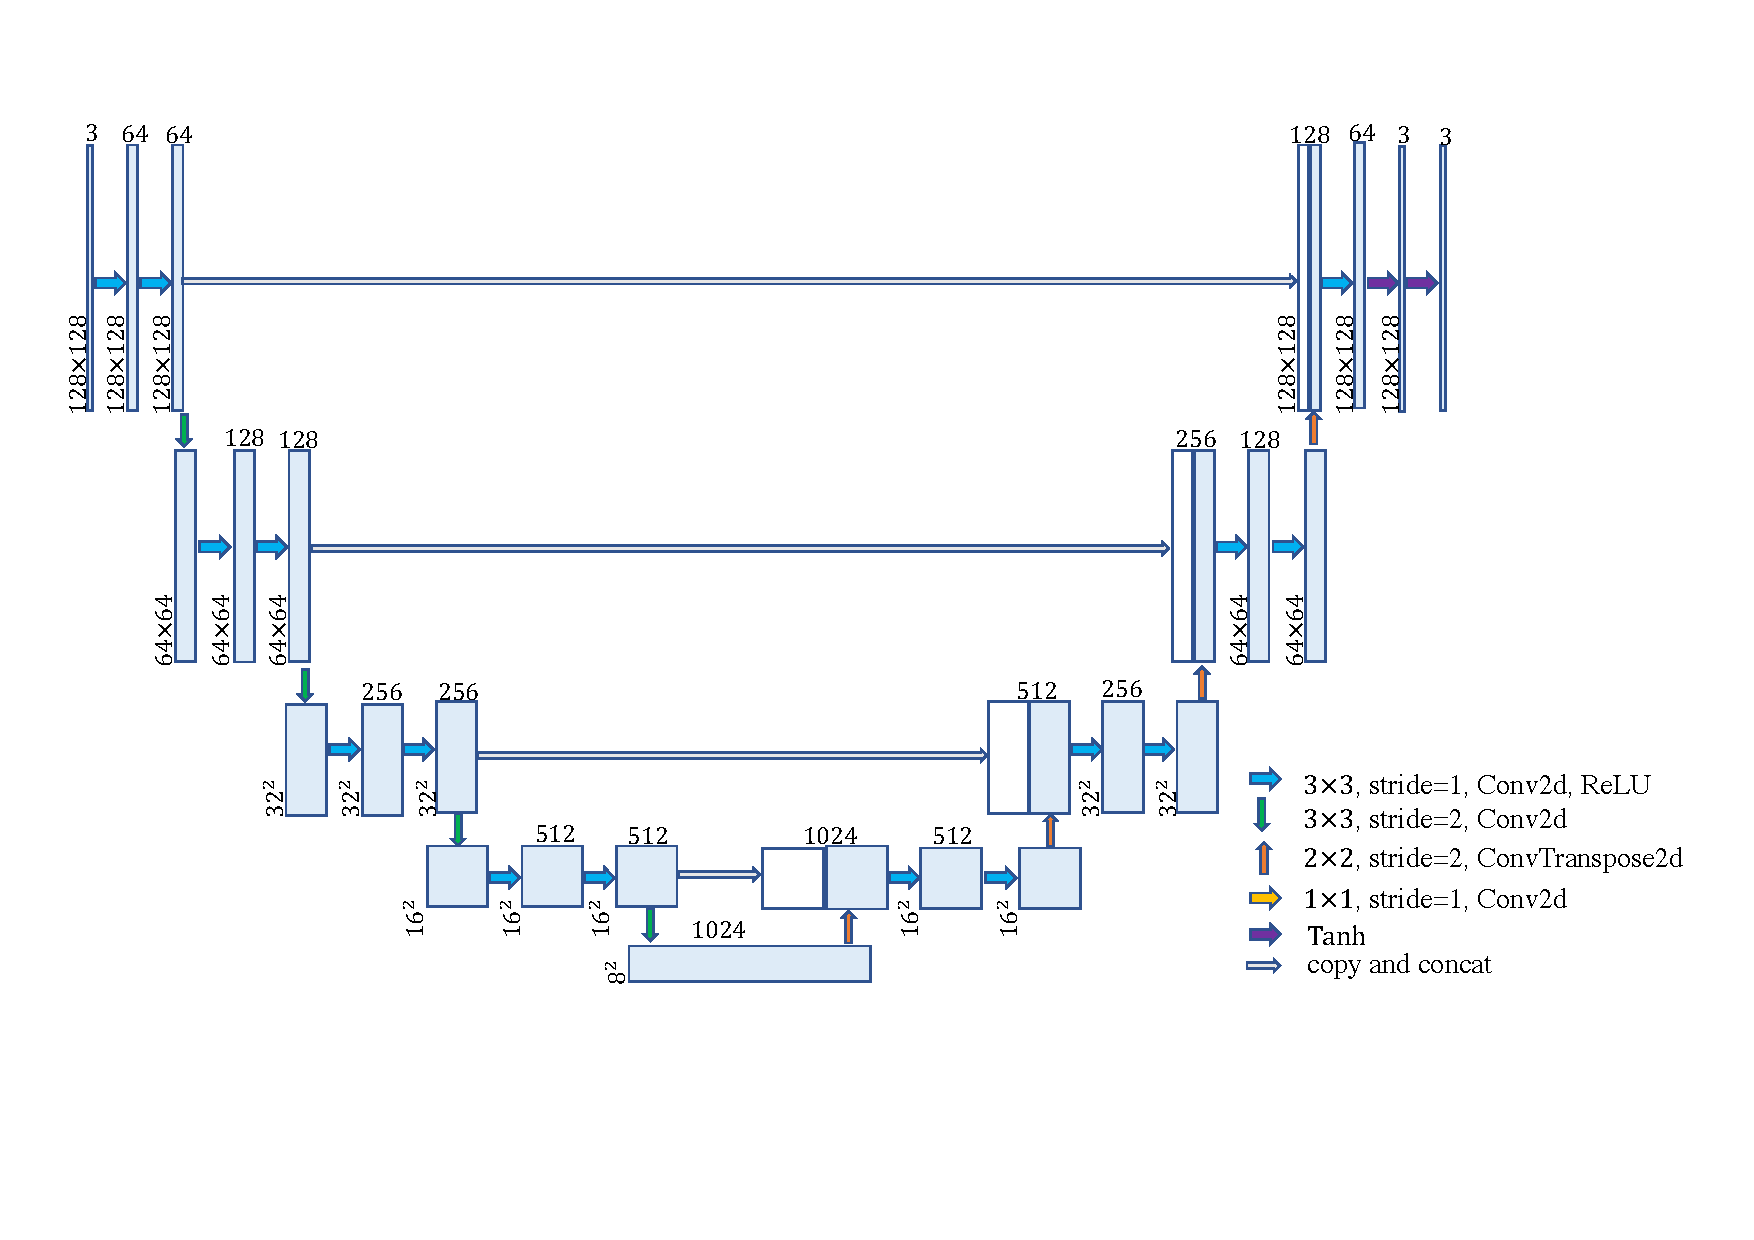
\includegraphics[width=1.0\textwidth]{figure/auto_encoder_architecture}
	\caption[本文编码器-解码器]{本文编码器-解码器。}
	\label{fig:auto_encoder_architecture}
\end{figure}
\vspace{-0.7cm}
\subsection{CNN分类器}\label{subsec:cnn_classifier_model}
选择CNN分类器时需要考虑的主要问题是如何选择一个分类性能优异的分类网络,最终本文CNN分类器选择ResNet网络~\cite{he2016deep}。一方面,ResNet系列网络具有良好的特性。加上编码器-解码器深度也较深,采用ResNet网络有利用避免梯度消失。另一方面,ResNet网络相对于VGG~\cite{simonyan2014very}等网络,参数量较少,计算开销较小。而相对于DenseNet~\cite{huang2017densely}、Inception~\cite{Szegedy2015RethinkingTI}等网络,ResNet模型结构较为简单、易于理解。本文CNN分类器的模型结构如图\ref{subfig:classifier_architecture}所示,可以发现,CNN分类器与原始ResNet-18相比没有作出较大改变,大部分卷积层(除跨层外)之后都会接上BatchNormalization层~\cite{ioffe2015batch}和ReLU激活函数,只是用3$\times$3卷积层代替了原始7$\times$7卷积层。这是因为原始ResNet-18的输入图像尺寸大小为224$\times$224,而本文CNN分类器的输入图像尺寸大小为128$\times$128。对于ResNet-18中的跨层连接,如果输入维度和输出维度相同,则直接相加(图\ref{subfig:classifier_architecture}中橘黄色折线);如果输入维度和输出维度不一样,本文将使用卷积核大小为1$\times$1、步长为2的卷积层将特征图尺寸减半(\ref{subfig:classifier_architecture}中蓝色折线),同时将通道数加倍。为了在跨层中保持尽量避免梯度消失问题和提高训练速度,本文同样在1$\times$1卷积层后接上BatchNormalization层。最后经过全局均值池化层的特征图送入输出维度为1的全连接层以处理二分类问题。
\begin{figure}[h!]
	\centering
	\begin{subfigure}{0.3\textwidth}
		\centering
		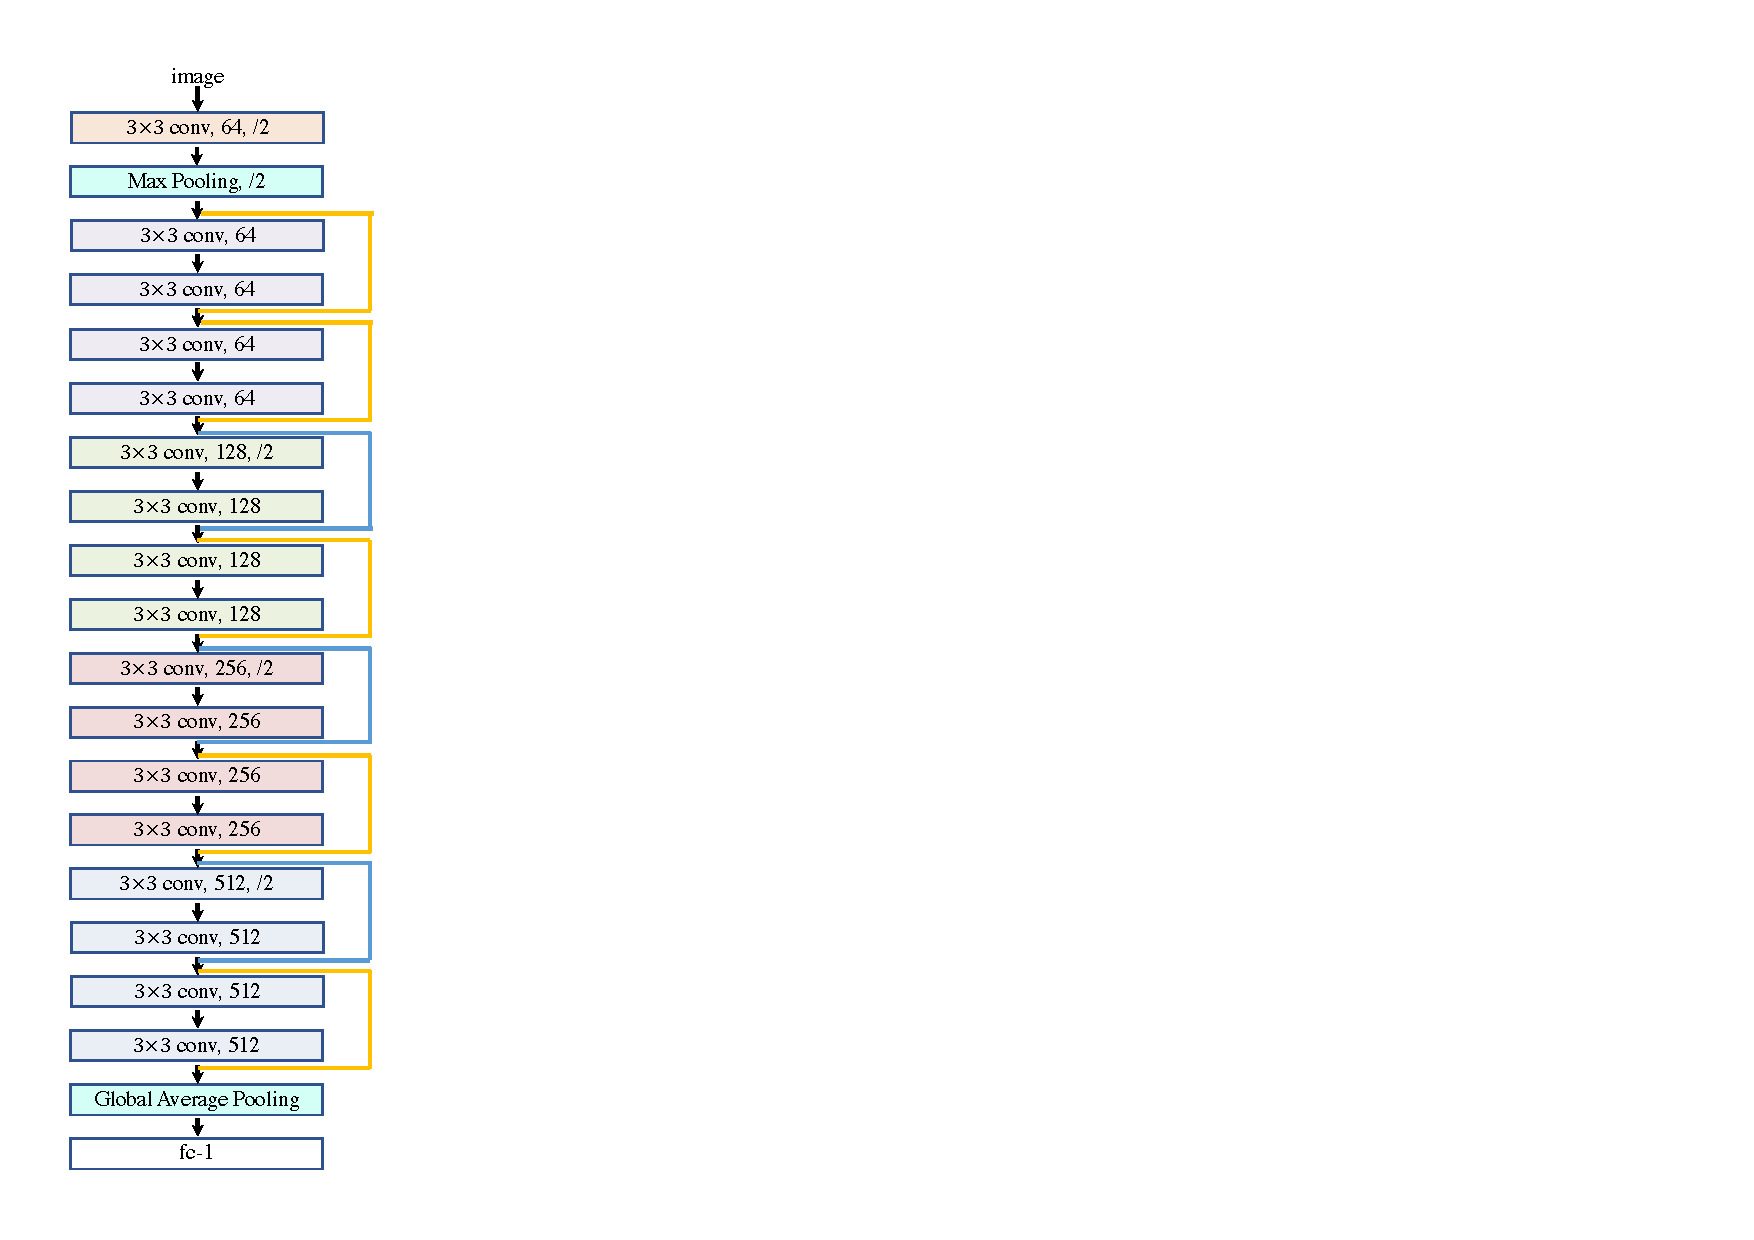
\includegraphics[width=1.0\textwidth]{figure/classifier_architecture.pdf}
		\caption{本文CNN分类器。}
		\label{subfig:classifier_architecture}
	\end{subfigure}
	\qquad\qquad\qquad\qquad
	\begin{subfigure}{0.348\textwidth}
		\centering
		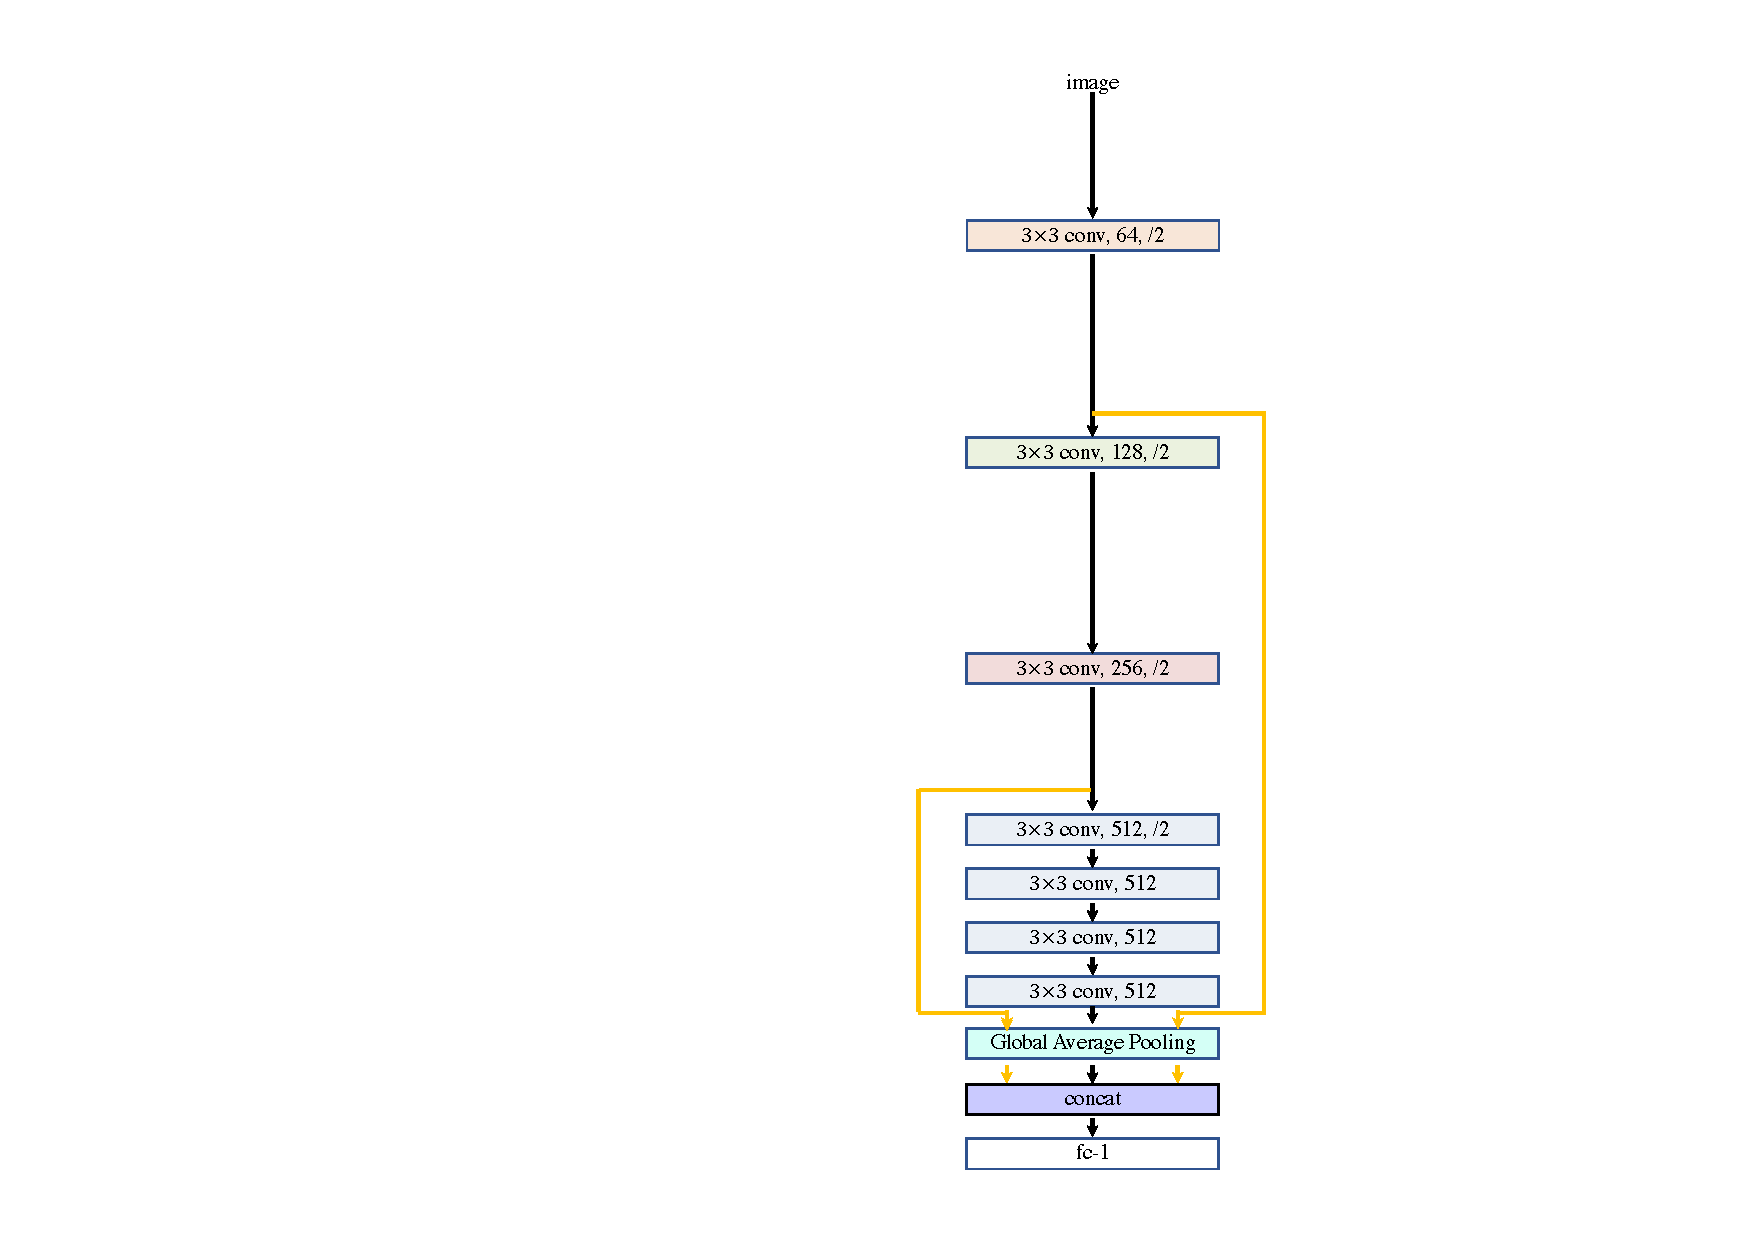
\includegraphics[width=1.0\textwidth]{figure/discrimintor_architecture.pdf}
		\caption{本文判别器。}
		\label{subfig:discrimintor_architecture}
	\end{subfigure}
	\caption[本文CNN分类器和判别器]{本文CNN分类器和判别器。CNN分类器网络和判别器网络的输入图像尺寸大小均为128$\times$128。子图\ref{subfig:classifier_architecture}中的蓝色折线表示可将输入尺寸大小减半、通道数加倍的跨层连接,子图\ref{subfig:discrimintor_architecture}和子图\ref{subfig:classifier_architecture}中的橘黄色折线表示恒等跨层连接。}
	\label{mul_fig:classifier_and_discrimintor_architecture}
\end{figure}
\subsection{判别器}\label{subsec:discrimintor_model}
本小节将详细介绍本文判别器的模型结构。如图\ref{subfig:discrimintor_architecture}所示,不难发现,卷积层(卷积核大小为3$\times$3)、BatchNormalization层和Leaky ReLU激活函数~\cite{maas2013rectifier}(负斜率为0.2)共同组成了本文判别器网络的基本单元。如图\ref{subfig:discrimintor_architecture},对于前4个卷积层,本文采用步长为2的3$\times$3卷积层达到下采样的目的,与此同时,随着特征图尺寸不断减小,卷积核的数量也以2倍关系增长(卷积核数量基数为64);对于第5-7个卷积层,卷积操作的步长为1,特征图尺寸不会发生变化,同时卷积核数量也不发生改变。最后,第一个下采样卷积层的特征图输出、最后一个下采样卷积层的特征图输出以及最后一个卷积层的特征图输出在经过全局均值池化层之后再进行拼接操作(图中concat操作),来融合低分辨率但语义强的特征(最后一个卷积层的特征图输出)和高分辨率但语义弱的特征(第一个下采样卷积层的特征图输出和最后一个下采样卷积层的特征图输出),最后将特征图送入输出维度为1全连接层。不难发现,判别器网络结构由下采样卷积层层数和卷积层总层数共同决定。在上文提到的诸多GAN中,由于训练WGAN-GP~\cite{gulrajani2017improved}时梯度相对比较稳定,不易发生梯度消失,损失函数对训练过程也有指示作用,故本文选用WGAN-GP,注意此时判别器不再是二分类器,而是去拟合Wasserstein-1距离的回归器,故判别器最后一层全连接层之后也没有Sigmoid激活函数。

本文参考了特征金字塔~\cite{lin2017feature},本文判别器和与普通GAN中的判别器相比,最主要的改动是增加了跨层结构。该结构通过从上而下的跨层连接,将网络中的低分辨率但语义强的特征图和高分辨率但语义弱的特征图融合起来,这种多尺度特征图相互融合的设计最初用于解决物体检测中小物体在连续下采样过程中容易被忽略的问题。由于浅层高分辨率但语义弱的特征中往往包含了与小物体相关的特征信息,故可通过这种多尺度特征图融合的方式,将与这些小物体相关的特征直接送到高层,与低分辨率但语义强的特征融合起来,使得各种大小不一的物体都能被CNN检测到。而医学影像中广泛分布的疾病标记物也有这种特点,而且疾病标记物的形状通常是不确定的、大小各异,并且数量往往不是一个,而是多个。因此,如果比较这些大小不一的疾病标记物,也会发现有些疾病标记物属于大物体,而另外一些疾病标记物属于小物体,甚至还会存在一些医生都难以察觉到的微小疾病标记物。也就是说,这种在物体检测任务中出现的小物体难以被发现的难题在医学影像领域的疾病标记物定位问题中不光存在,而且更加突出。这也是本文判别器中加入跨层结构的原因所在。

\section{训练策略与损失函数}\label{sec:loss_func_training_stragies}
在\ref{sec:model_architecture_intro}小节中,本文介绍了本文提出的方法的模型结构以及子模块(CNN分类器、判别器和编码器-解码器)的模型结构。本节内容将在此基础上介绍本文提出的模型的训练策略(见\ref{subsec:traing_stragies}小节)以及损失函数(见\ref{subsec:loss_func}小节)。
\subsection{训练策略}\label{subsec:traing_stragies}
如\ref{subsec:model_architecture}所描述的那样,本文提出的网络模型中共有三个子模块:编码器-解码器、CNN分类器和判别器。根据\ref{sec:idea_thinking}小节描述的解决思路:编码器-解码器是一种无监督模型,本身并没有识别疾病标记物的能力,因此需要借助其他模块来指导编码器-解码器,使得编码器-解码器能够识别异常图像中的疾病标记物,进而编码器-解码器通过编码阶段和解码阶段来去除异常图像中的疾病标记物,这也是本文提出的模型中引入CNN分类器和判别器的原因。换句话说,本文希望CNN分类器通过完成分类任务来迫使编码器-解码器具有一定的识别疾病标记物的能力,尽量去除异常图像中的疾病标记物。一旦CNN分类器出现无法彻底去除(部分去除)疾病标记物的情况,即此时异常图像中仍有比较微小的、难以察觉的疾病标记物存在,这时通过训练生成对抗网络让编码器-解码器的输出图像更像真实正常图像来迫使编码器-解码器进一步完全去除异常图像中的疾病标记物,故本文将在第一步中训练CNN分类器和编码器-解码器,在第二步中训练由编码器-解码器和判别器组成的GAN。综上所述,本文提出的两步训练策略如下:

1)固定判别器,更新编码器-解码器和CNN分类器(以下简称“第一步”):这一步将编码器-解码器和CNN分类器联合起来训练,更新编码器-解码器和CNN分类器。这一步旨在让CNN分类器完成一个分类任务,来迫使编码器-解码器能在异常图像输入时尽量去除异常图像中疾病标记物。注意此时GAN中的判别器并未参与训练过程。

2)固定CNN分类器,更新编码器-解码器和判别器(以下简称“第二步”):第二步将编码器-解码器和判别器组合起来训练,其训练过程与WGAN-GP一致,分为两个子步骤,按照先后顺序依次更新判别器(注意固定编码器-解码器)和编码器-解码器(注意固定判别器)。我们希望编码器-解码器在经过对抗训练(真实正常图像 vs. 编码器-解码器的输出图像)之后能进一步彻底去除第一步中未能去除的疾病标记物,生成异常图像对应的“正常”图像。注意此时CNN分类器并未参与训练过程。

注意,默认每训练一批数据(Mini-batch)后上述两个步骤就会交替训练一次,这种频繁的交替训练可能会造成GAN在训练的过程中发生震荡,为避免这种问题,可以选择训练所有数据(Epoch)后再将以上两步骤交替训练一次。为了让CNN分类器在初始化情况下就具备一定识别疾病标记物的能力,以期望在第一步中,CNN分类器能指导编码器-解码器尽可能多地去除图像中的疾病标记物,可先将第一步连续训练多次或者利用预训练参数初始化CNN分类器。对于纹理结构比较丰富的医学图像(比如,眼底图像),可用梯度算子(比如,索贝尔算子\footnote{https://en.wikipedia.org/wiki/Sobel\_operator}和拉普拉斯算子\footnote{https://en.wikipedia.org/wiki/Laplace\_operator})检测边缘,将其作为输入图像中的像素点的权重,以便于编码器-解码器能更加容易地重构这些复杂的纹理结构。除此之外,同样可以使用预训练参数初始化编码器-解码器来达到这一目的。

待本文提出的模型训练结束之后,异常图像中的疾病标记物的位置就可以通过编码器-解码器的输入与输出之差给出了。而输入图像的标签,可以由CNN分类器给出。
\subsection{损失函数}\label{subsec:loss_func}
接下来,本小节将介绍本文提出的模型在处理疾病标记物定位任务时的损失函数,不妨用$G$表示编码器-解码器,用$D$表示判别器,用$C$表示CNN分类器。设疾病标记物定位问题的损失函数为${L}$,本文将$L$定义为:
\begin{equation}\label{equ:model_loss_func}
\min _{G, C} \max _{D} \;\; L=L_{GAN}(D, G)+\lambda_{1} L_{C E}(C, G)+\lambda_{2} L_{E D}(G).
\end{equation}
其中,$L_{GAN}(D,G)$表示生成对抗网络的损失函数(本文使用WGAN-GP),$L_{CE}(C, G)$表示CNN分类器的交叉熵损失函数,$L_{E D}(G)$是约束编码器-解码器的损失函数(本文使用L1损失函数),用于强调输入和输出之间的相似性,$\lambda{1}$和$\lambda_{2}$是两个超参数,用于平衡各个损失函数之间的权重。注意$L_{E D}(G)$这一项是不可缺少的,一旦缺少($\lambda_{2}=0$),在CNN分类器和判别器的指导下,编码器-解码器很可能在修改疾病标记物所在区域的同时还会修改正常区域,这将导致不可避免地出现假阳现象。

接下来,本文将给出每个步骤训练时的损失函数。根据等式\ref{equ:model_loss_func}和\ref{subsec:traing_stragies}小节中描述的训练策略,本文可进一步分别给出本文两步训练策略对应的损失函数。设第一步和第二步的损失函数分别为$L_1$和$L_2$,则第一步训练的损失函数$L_1$定义为:
\begin{equation}
\min_{G, C} \;\; L_{1}=\lambda_1 L_{CE}(C,G) + \lambda_2 L_{ED}(G).
\end{equation}
在第二步中,编码器-解码器和判别器组成GAN,则损失函数$L_2$可定义为:
\begin{equation}
\min_{G} \max_D \;\; L_{2}= L_{GAN}(D,G) + \lambda_2 L_{ED}(G).
\end{equation}

到这里,本文将模型方法相关内容叙述都已描述完毕。为了更为清晰表示其训练过程及其损失函数,与之对应的算法过程描述如算法\ref{alg:net}所示。从算法\ref{alg:net}也可以看出,本文中GAN选用的是WGAN-GP。

\begin{algorithm}[h!]
	\SetAlgoLined
	\caption{本文提出的模型的训练过程。}
	\label{alg:net}
	\SetKwInOut{Input}{Input}\SetKwInOut{Output}{output}
	\Input{The gradient penalty coefficient $\lambda$, learning rate $\alpha$, batch size $m$, hyperparameters $\lambda _1$ and $\lambda _2$, encoder-decoder's parameters $\vv{\theta} _g$, classifier's parameters $\vv{\theta} _c$, discriminator's parameters $\vv{\theta} _d$, maximum iterations $K$.}
	\nl \For{$k\leftarrow 1$ \KwTo $K$}{
		%reference: http://mlg.ulb.ac.be/files/algorithm2e.pdf
		\nl
		Sample a batch $\{\ve{x}^{(i)}\}_{i=1}^{m}$ from the normal dataset, and a batch $\{\ve{z}^{(i)}\}_{i=1}^{m}$ from the abnormal dataset; collect both to get batch $\ve{y}=\{\ve{y}^{(i)}\}_{i=1}^{2m}$, and their image-level labels $\ve{l}=\{\ve{l}^{(i)}\}_{i=1}^{2m}$.\\
		\nl	$L(\ve{y},\ve{l};\vv{\theta})$ $\leftarrow \lambda _1$[$\frac{1}{2m}\sum_{i=1}^{2m}$$L_{CE}(C(G(\ve{y}^{(i)};\vv{\theta});\vv{\theta}), \ve{l}^{(i)})$] \\
		\qquad \qquad \, \, \, $+$$\lambda _2[\frac{1}{2m}\sum_{i=1}^{2m}L_{ED}(G(\ve{y}^{(i)};\vv{\theta}),\ve{y}^{(i)})]$  \\
		\nl	$\vv{\theta} _g$$\leftarrow Adam(\nabla _{\vv{\theta} _g} L(\ve{y},\ve{l};\vv{\theta}), \vv{\theta} _g, \alpha)$
		\tcp*{minimize G}
		\nl	$\vv{\theta} _c$$\leftarrow Adam(\nabla _{\vv{\theta} _c} L(\ve{y},\ve{l};\vv{\theta}), \vv{\theta} _c, \alpha)$
		\tcp*{minimize C}
		\nl	$\hat{\ve{x}}^{(i)}\leftarrow \eta \ve{x}^{(i)} + (1-\eta)G(\ve{z}^{(i)};\vv{\theta})$, $\eta\sim \text{U}(0, 1)$ ;\\
		
		$L(\ve{x},\hat{\ve{x}},\ve{z};\vv{\theta})$ $\leftarrow $$\frac{1}{m}\sum_{i=1}^{m}$$[D(G(\ve{z}^{(i)};\vv{\theta});\vv{\theta})-$$D(\ve{x}^{(i)};\vv{\theta})$\\ \qquad \qquad \qquad \qquad \quad \,\, $+\lambda \left(\left\|\nabla_{\hat{\ve{x}}^{(i)}} D(\hat{\ve{x}}^{(i)};\vv{\theta})\right\|_{2}-1\right)^{2}]$ \\
		\nl	$\vv{\theta} _d$$\leftarrow Adam(\nabla _{\vv{\theta} _d} L(\ve{x},\hat{\ve{x}},\ve{z};\vv{\theta}), \vv{\theta} _d, \alpha)$ 
		\tcp*{maximize D}
		$L(\ve{x}, \ve{z}; \vv{\theta})\leftarrow -\frac{1}{m}\sum_{i=1}^{m}D(G(\ve{z}^{(i)};\vv{\theta});\vv{\theta})+\lambda_2[\frac{1}{m}\sum_{i=1}^{m}L_{ED}(G(\ve{x}^{(i)};\vv{\theta}),\ve{x}^{(i)})$
		\\ \qquad \qquad \qquad \qquad \qquad \qquad \qquad \qquad \qquad \,
		$+\frac{1}{m}\sum_{i=1}^{m}L_{ED}(G(\ve{z}^{(i)};\vv{\theta}),\ve{z}^{(i)}))]$\\
		\nl	$\vv{\theta} _g$$\leftarrow Adam(\nabla _{\vv{\theta} _g} L(\ve{x}, \ve{z}; \vv{\theta}), \vv{\theta} _g, \alpha)$ 
		\tcp*{minimize G}
}
\end{algorithm}
\section{本章小结}\label{sec:chapter3_summary}
本章内容主要围绕本文提出的疾病标记物自动定位模型展开。本文在\ref{sec:idea_thinking}小节中介绍了研究问题和解决思路。随后,本文在\ref{sec:model_architecture_intro}小节阐述本文提出的模型的整体结构,本文提出的模型共包括三个子模块:编码器-解码器、CNN分类器和判别器。该模型以编码器-解码器为骨架网络,以CNN分类器和判别器为辅助角色指导编码器-解码器,使编码器-解码器能通过编码阶段和解码阶段去除疾病标记物。编码器-解码器和判别器组成了GAN。给定任意一张输入图像,我们希望通过CNN分类器给出其类别(正常/异常),对于异常图像,通过编码器-解码器的输入和输出之差来给出疾病标记物的精确位置。接着在\ref{subsec:encoder_decoder_model}小节、\ref{subsec:cnn_classifier_model}小节和\ref{subsec:discrimintor_model}小节中分别介绍了编码器-解码器、CNN分类器和判别器的网络结构,以期读者不仅能对本文提出的模型有宏观上的理解,还不缺乏子模块细节上的详实说明。随后,本文在\ref{sec:loss_func_training_stragies}小节中给出了本文提出的模型的两步训练策略(见\ref{subsec:traing_stragies}小节)以及对应的损失函数(见\ref{subsec:loss_func}小节)。为了方便读者进一步理解本文提出的训练策略,在算法\ref{alg:net}中,本文还用形式化语言描述了本文提出的模型的训练过程。到此,本文提出的方法的相关介绍结束,我们将在第\ref{sec:experiments}章和第\ref{sec:multi_classes}章中介绍实验验证。
